\subsection*{Greedy Single Source Shortest Path}

\subsubsection*{Process}

The answer to this problem can be derived using Dijkstra's algorithm. In the following table, $u$ refers to the node of context for each iteration of the loop, while all other values represent the distance from node 1.

\begin{table}[H]
\begin{center}
\begin{tabular}{c|ccccccccc}
$u$ & 
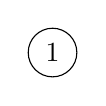
\begin{tikzpicture}[auto,node distance=2.5cm,main node/.style={circle,draw}] \node[main node] (1) {1}; \end{tikzpicture} & 
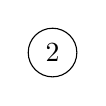
\begin{tikzpicture}[auto,node distance=2.5cm,main node/.style={circle,draw}] \node[main node] (2) {2}; \end{tikzpicture} & 
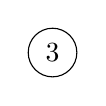
\begin{tikzpicture}[auto,node distance=2.5cm,main node/.style={circle,draw}] \node[main node] (3) {3}; \end{tikzpicture} & 
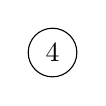
\begin{tikzpicture}[auto,node distance=2.5cm,main node/.style={circle,draw}] \node[main node] (4) {4}; \end{tikzpicture} & 
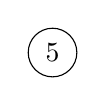
\begin{tikzpicture}[auto,node distance=2.5cm,main node/.style={circle,draw}] \node[main node] (5) {5}; \end{tikzpicture} & 
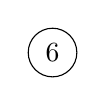
\begin{tikzpicture}[auto,node distance=2.5cm,main node/.style={circle,draw}] \node[main node] (6) {6}; \end{tikzpicture} & 
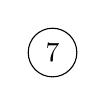
\begin{tikzpicture}[auto,node distance=2.5cm,main node/.style={circle,draw}] \node[main node] (7) {7}; \end{tikzpicture} & 
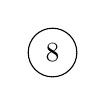
\begin{tikzpicture}[auto,node distance=2.5cm,main node/.style={circle,draw}] \node[main node] (8) {8}; \end{tikzpicture} & 
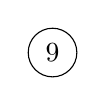
\begin{tikzpicture}[auto,node distance=2.5cm,main node/.style={circle,draw}] \node[main node] (9) {9}; \end{tikzpicture} \\
\hline \\[-0.97em]
  & 0 &  $\infty$  &  $\infty$  &  $\infty$  &  $\infty$  &  $\infty$  &   $\infty$  &   $\infty$  &  $\infty$  \\
\hline \\[-0.9em]
1 & 0 & \textbf{2} & \textbf{2} &  $\infty$  &  $\infty$  &  $\infty$  &   $\infty$  &   $\infty$  & \textbf{7} \\
2 & 0 &         2  &         2  &  $\infty$  & \textbf{5} &  $\infty$  &   $\infty$  &   $\infty$  &         7  \\
3 & 0 &         2  &         2  & \textbf{3} &         5  & \textbf{6} &   $\infty$  &   $\infty$  &         7  \\
4 & 0 &         2  &         2  &         3  &         5  &         6  &   $\infty$  &   $\infty$  & \textbf{5} \\
5 & 0 &         2  &         2  &         3  &         5  &         6  & \textbf{10} &   $\infty$  &         5  \\
9 & 0 &         2  &         2  &         3  &         5  &         6  &         10  &   $\infty$  &         5  \\
6 & 0 &         2  &         2  &         3  &         5  &         6  &         10  & \textbf{12} &         5  \\
7 & 0 &         2  &         2  &         3  &         5  &         6  &         10  & \textbf{11} &         5  \\
8 & 0 &         2  &         2  &         3  &         5  &         6  &         10  &         11  &         5  \\
\end{tabular}
\end{center}
\caption{Distance Trace of Dijkstra's Single Source Shortest Path Algorithm}
\end{table}

\subsubsection*{Solution}

\begin{figure}[H]
\begin{center}
\adjustbox{valign=t}{
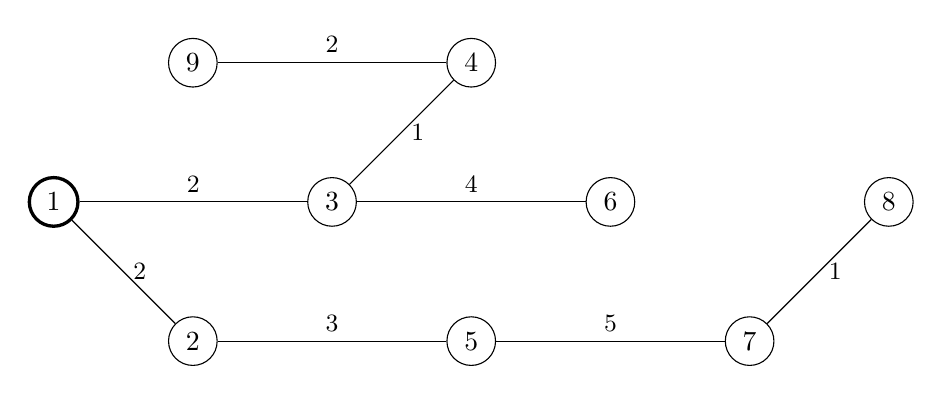
\begin{tikzpicture}[auto,node distance=2.5cm,main node/.style={circle,draw}]
  \node[main node, line width=1.2pt] (1) {1};
  \node[main node] (2) [below right of=1] {2};
  \node[main node] (3) [above right of=2] {3};
  \node[main node] (4) [above right of=3] {4};
  \node[main node] (5) [below right of=3] {5};
  \node[main node] (6) [below right of=4] {6};
  \node[main node] (7) [below right of=6] {7};
  \node[main node] (8) [above right of=7] {8};
  \node[main node] (9) [above right of=1] {9};
  
  \path[every node/.style={font=\small}]
    (3) edge node [right] {1} (4)
    (7) edge node [right] {1} (8)
    (1) edge node [right] {2} (2)
    (1) edge node [above] {2} (3)
    (9) edge node [above] {2} (4)
    (2) edge node [above] {3} (5)
    (3) edge node [above] {4} (6)
    (5) edge node [above] {5} (7);
\end{tikzpicture}
} \\[10pt]
\end{center}
\caption{Dijkstra's Single Source Shortest Path Tree}
\end{figure}